\section{Experimental Results}
\label{sec:experimental_results}

This section presents the results of our experiments structured around the four research questions defined in Section~\ref{sec:introduction}. We evaluate models on both tasks using the metrics described in Section~\ref{subsec:evaluation}.


\subsection{RQ1: Transformer Models vs. Traditional Baselines}
\label{subsec:rq1}

We first establish baseline performance using classical machine learning approaches before evaluating transformer-based models.

\paragraph{Baseline Results (Task 1).}
Table~\ref{tab:task1-baselines} presents the performance of traditional baselines on Task~1. The majority class baseline achieves 66.9\% test accuracy but only 26.7\% macro F1, indicating it simply predicts the dominant ``Ambivalent'' class. Both TF-IDF-based approaches substantially outperform this naive baseline, with Linear SVM achieving the best baseline performance (60.7\% accuracy, 45.5\% macro F1 on test).

\begin{table}[t]
    \centering
    \small
    \begin{tabular}{lcc}
        \toprule
        \textbf{Model}        & \textbf{Val F1 (\%)} & \textbf{Test F1 (\%)} \\
        \midrule
        Majority             & 24.8 & 26.7 \\
        Logistic Regression  & 57.7 & 44.6 \\
        Linear SVM           & \textbf{58.8} & \textbf{45.5} \\
        \bottomrule
    \end{tabular}
    \caption{Baseline results for Task~1 (Clarity classification). Scores are macro F1.}
    \label{tab:task1-baselines}
\end{table}

\paragraph{Baseline Results (Task 2).}
Task~2 proves more challenging due to severe class imbalance (Table~\ref{tab:class-dist}). The majority baseline achieves only 30.4\% validation accuracy and 5.2\% macro F1, reflecting the 9-way classification difficulty. TF-IDF approaches show modest improvements, with Linear SVM reaching 33.0\% validation accuracy and 30.2\% macro F1. On the multi-annotator test set, SVM achieves 35.4\% accuracy under the ``match any annotator'' criterion.

\begin{table}[t]
    \centering
    \small
    \begin{tabular}{lcc}
        \toprule
        \textbf{Model}        & \textbf{Val F1 (\%)} & \textbf{Test Acc (\%)$^\dagger$} \\
        \midrule
        Majority             & 5.2  & 29.5 \\
        Logistic Regression  & 29.7 & 32.1 \\
        Linear SVM           & \textbf{30.2} & \textbf{35.4} \\
        \bottomrule
    \end{tabular}
    \caption{Baseline results for Task~2 (Evasion classification). $^\dagger$Multi-annotator test accuracy.}
    \label{tab:task2-baselines}
\end{table}

\paragraph{Transformer Model Results.}
Table~\ref{tab:transformer-results} shows that transformer models substantially outperform baselines on both tasks. Figure~\ref{fig:task-comparison} visualizes the performance comparison across all models for both tasks. On Task~1, BERT achieves 67.2\% test accuracy and 56.6\% macro F1, representing a \textbf{+11.1 percentage point} improvement in macro F1 over the best baseline (Linear SVM: 45.5\%). DistilBERT performs nearly as well (66.6\% accuracy, 56.0\% macro F1) while being more parameter-efficient. ALBERT shows lower Task~1 performance (62.3\% accuracy, 51.3\% macro F1) but interestingly performs best on the hierarchy-based clarity metric (48.9\% macro F1 when mapping evasion predictions to clarity).

For Task~2, transformer models show significant improvements over baselines in multi-annotator test accuracy. ALBERT achieves the highest test accuracy (44.5\%), followed by BERT (42.2\%) and DistilBERT (41.6\%). These represent \textbf{+9.1 to +6.2 percentage point} improvements over the Linear SVM baseline (35.4\%).

\begin{table}[t]
    \centering
    \small
    \begin{tabular}{lccc}
        \toprule
        \textbf{Model} & \textbf{T1 F1 (\%)} & \textbf{T2 Acc (\%)$^\dagger$} & \textbf{Hier.(\%)$^\ddagger$} \\
        \midrule
        DistilBERT & 56.0 & 41.6 & 45.0 \\
        BERT       & \textbf{56.6} & 42.2 & 44.6 \\
        ALBERT     & 51.3 & \textbf{44.5} & \textbf{48.9} \\
        \bottomrule
    \end{tabular}
    \caption{Transformer model results (LR=3e--5, WD=0.0). T1 = Task~1 test macro F1, T2 = Task~2 test accuracy. $^\dagger$Multi-annotator evaluation. $^\ddagger$Evasion$\rightarrow$clarity via taxonomy.}
    \label{tab:transformer-results}
\end{table}

\begin{figure}[t]
    \centering
    \resizebox{\columnwidth}{!}{%
        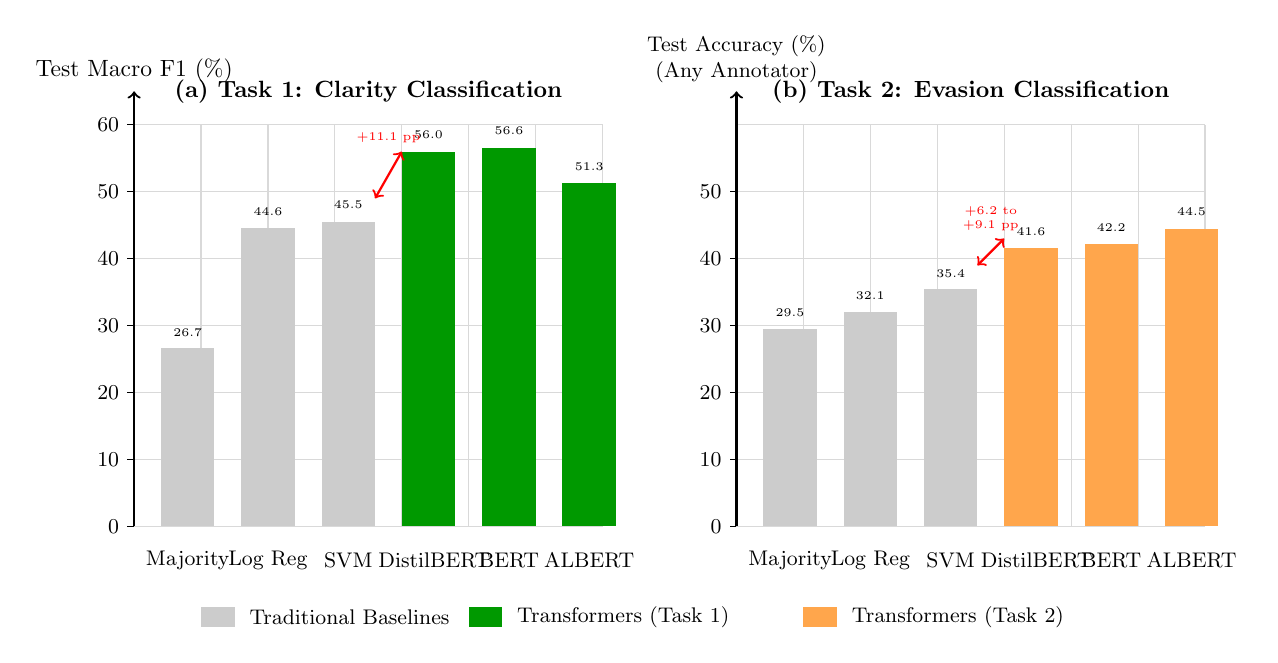
\begin{tikzpicture}[scale=0.85, transform shape]
    % Task 1: Clarity Classification
    \begin{scope}
        % Title
        \node[font=\bfseries] at (3.5, 6.5) {(a) Task 1: Clarity Classification};
        
        % Grid
        \draw[gray!30] (0,0) grid[xstep=1, ystep=1] (7,6);
        
        % Y-axis
        \draw[thick,->] (0,0) -- (0,6.5) node[above] {Test Macro F1 (\%)};
        \foreach \y in {0,10,20,30,40,50,60}
            \draw (0,\y/10) -- (-0.1,\y/10) node[left, font=\small] {\y};
        
        % X-axis with model names
        \node[font=\small, text width=1.5cm, align=center] at (0.8,-0.5) {Majority};
        \node[font=\small, text width=1.5cm, align=center] at (2,-0.5) {Log Reg};
        \node[font=\small, text width=1.5cm, align=center] at (3.2,-0.5) {SVM};
        \node[font=\small, text width=1.5cm, align=center] at (4.4,-0.5) {DistilBERT};
        \node[font=\small, text width=1.5cm, align=center] at (5.6,-0.5) {BERT};
        \node[font=\small, text width=1.5cm, align=center] at (6.8,-0.5) {ALBERT};
        
        % Bars - Baselines (gray)
        \fill[gray!40] (0.4, 0) rectangle (1.2, 2.67);  % Majority: 26.7%
        \fill[gray!40] (1.6, 0) rectangle (2.4, 4.46);  % Log Reg: 44.6%
        \fill[gray!40] (2.8, 0) rectangle (3.6, 4.55);  % SVM: 45.5%
        
        % Bars - Transformers (green)
        \fill[green!60!black] (4.0, 0) rectangle (4.8, 5.60);   % DistilBERT: 56.0%
        \fill[green!60!black] (5.2, 0) rectangle (6.0, 5.66);   % BERT: 56.6%
        \fill[green!60!black] (6.4, 0) rectangle (7.2, 5.13);   % ALBERT: 51.3%
        
        % Value labels
        \node[font=\tiny] at (0.8, 2.9) {26.7};
        \node[font=\tiny] at (2.0, 4.7) {44.6};
        \node[font=\tiny] at (3.2, 4.8) {45.5};
        \node[font=\tiny] at (4.4, 5.85) {56.0};
        \node[font=\tiny] at (5.6, 5.91) {56.6};
        \node[font=\tiny] at (6.8, 5.38) {51.3};
        
        % Improvement annotation
        \draw[thick, red, <->] (3.6, 4.9) -- (4.0, 5.6);
        \node[font=\tiny, red, text width=1.2cm, align=center] at (3.8, 5.8) {+11.1 pp};
    \end{scope}
    
    % Task 2: Evasion Classification
    \begin{scope}[xshift=9cm]
        % Title
        \node[font=\bfseries] at (3.5, 6.5) {(b) Task 2: Evasion Classification};
        
        % Grid
        \draw[gray!30] (0,0) grid[xstep=1, ystep=1] (7,6);
        
        % Y-axis
        \draw[thick,->] (0,0) -- (0,6.5) node[above, text width=3cm, align=center, font=\small] {Test Accuracy (\%)\\(Any Annotator)};
        \foreach \y in {0,10,20,30,40,50}
            \draw (0,\y/10) -- (-0.1,\y/10) node[left, font=\small] {\y};
        
        % X-axis with model names
        \node[font=\small, text width=1.5cm, align=center] at (0.8,-0.5) {Majority};
        \node[font=\small, text width=1.5cm, align=center] at (2,-0.5) {Log Reg};
        \node[font=\small, text width=1.5cm, align=center] at (3.2,-0.5) {SVM};
        \node[font=\small, text width=1.5cm, align=center] at (4.4,-0.5) {DistilBERT};
        \node[font=\small, text width=1.5cm, align=center] at (5.6,-0.5) {BERT};
        \node[font=\small, text width=1.5cm, align=center] at (6.8,-0.5) {ALBERT};
        
        % Bars - Baselines (gray)
        \fill[gray!40] (0.4, 0) rectangle (1.2, 2.95);  % Majority: 29.5%
        \fill[gray!40] (1.6, 0) rectangle (2.4, 3.21);  % Log Reg: 32.1%
        \fill[gray!40] (2.8, 0) rectangle (3.6, 3.54);  % SVM: 35.4%
        
        % Bars - Transformers (orange)
        \fill[orange!70] (4.0, 0) rectangle (4.8, 4.16);   % DistilBERT: 41.6%
        \fill[orange!70] (5.2, 0) rectangle (6.0, 4.22);   % BERT: 42.2%
        \fill[orange!70] (6.4, 0) rectangle (7.2, 4.45);   % ALBERT: 44.5%
        
        % Value labels
        \node[font=\tiny] at (0.8, 3.2) {29.5};
        \node[font=\tiny] at (2.0, 3.45) {32.1};
        \node[font=\tiny] at (3.2, 3.78) {35.4};
        \node[font=\tiny] at (4.4, 4.4) {41.6};
        \node[font=\tiny] at (5.6, 4.46) {42.2};
        \node[font=\tiny] at (6.8, 4.7) {44.5};
        
        % Improvement annotation
        \draw[thick, red, <->] (3.6, 3.9) -- (4.0, 4.3);
        \node[font=\tiny, red, text width=1.2cm, align=center] at (3.8, 4.6) {+6.2 to\\+9.1 pp};
    \end{scope}
    
    % Legend
    \begin{scope}[yshift=-1.5cm]
        \fill[gray!40] (1,0) rectangle (1.5, 0.3);
        \node[right, font=\small] at (1.6, 0.15) {Traditional Baselines};
        
        \fill[green!60!black] (5,0) rectangle (5.5, 0.3);
        \node[right, font=\small] at (5.6, 0.15) {Transformers (Task 1)};
        
        \fill[orange!70] (10,0) rectangle (10.5, 0.3);
        \node[right, font=\small] at (10.6, 0.15) {Transformers (Task 2)};
    \end{scope}
\end{tikzpicture}

    }
    \caption{Performance comparison on both tasks.}
    \label{fig:task-comparison}
\end{figure}

\paragraph{Answer to RQ1.}
Transformer-based models \emph{consistently and substantially outperform} traditional TF-IDF + SVM baselines on both tasks. The improvement is particularly pronounced on Task~1 (clarity classification), where BERT shows a +11.1 pp gain in macro F1. On the more challenging Task~2 (evasion classification), transformers still achieve meaningful improvements of +6-9 pp in test accuracy, demonstrating their superior ability to capture semantic relationships between questions and answers.


\subsection{RQ2: Class Imbalance and Focal Loss}
\label{subsec:rq2}

Task~2 exhibits severe class imbalance (Table~\ref{tab:class-dist}), with the most frequent class (\textit{Explicit}, 30.5\%) being 13.3$\times$ more common than the least frequent (\textit{Partial/half-answer}, 2.3\%). To address this, we employed Focal Loss~\cite{lin2017focal} with $\gamma = 2.0$ for all Task~2 experiments, which down-weights easy examples to focus learning on hard cases.

\paragraph{Results.} Despite using Focal Loss, class imbalance significantly affects performance. There seems to be a strong correlation between class frequency and F1 scores: frequent classes (>400 samples) achieve F1 $\in$ [0.35, 0.45], while rare classes (<100 samples) achieve F1 $\in$ [0.05, 0.20]. The three rarest classes (\textit{Partial/half-answer}, \textit{Clarification}, \textit{Claims ignorance}) consistently score below F1=0.15.

Our Focal Loss-trained models outperform baselines by 2-4 percentage points in validation macro F1 (DistilBERT: 33.8\% vs. SVM: 30.2\%), but the fundamental challenge of insufficient training data for minority classes remains. Confusion analysis reveals systematic errors between semantically similar strategies (e.g., \textit{Implicit} $\leftrightarrow$ \textit{Dodging}), suggesting the fine-grained taxonomy may require additional context beyond question-answer pairs.

\subsection{RQ3: Architecture Comparison}
\label{subsec:rq3}

We compare three transformer architectures across performance and efficiency dimensions (Table~\ref{tab:efficiency}).

\begin{table}[t]
\centering
\small
\begin{tabular}{lrrr}
\toprule
\textbf{Model} & \textbf{Params} & \textbf{Time/epoch} & \textbf{T1 F1} \\
\midrule
DistilBERT & 66M & 6 min & 56.0\% \\
BERT & 110M & 10 min & 56.6\% \\
ALBERT & 12M & 8 min & 51.3\% \\
\bottomrule
\end{tabular}
\caption{Architecture comparison on T4 GPU. T1 F1 = Task~1 test macro F1.}
\label{tab:efficiency}
\end{table}

\textbf{DistilBERT} offers the best trade-off: it achieves 99\% of BERT's Task~1 performance (56.0\% vs. 56.6\% macro F1) while being 1.67$\times$ faster with 40\% fewer parameters. \textbf{BERT} achieves the highest Task~1 accuracy (67.2\%) but at greater computational cost. \textbf{ALBERT}, despite having only 12M parameters, achieves the best Task~2 test accuracy (44.5\%), suggesting parameter sharing benefits fine-grained classification, though it underperforms on Task~1.

For production deployment prioritizing inference speed, we recommend DistilBERT. For maximum Task~1 accuracy, BERT remains the best choice. ALBERT suits resource-constrained scenarios where Task~2 performance is critical.


\subsection{RQ4: LLM-Based Prompted Inference}
\label{subsec:llm-results}

We evaluate the zero-to-few-shot capabilities of Llama 3 across four configurations (0, 1, 3, and 9 shots). Results are summarized in Table~\ref{tab:llm_results} and Figure~\ref{fig:llama_scaling}.

\begin{table}[h]
\centering
\small
\begin{tabular}{lcccc}
\toprule
\textbf{Metric} & \textbf{0-Shot} & \textbf{1-Shot} & \textbf{3-Shot} & \textbf{9-Shot} \\
\midrule
Clarity Acc. & 0.455 & \textbf{0.682} & 0.542 & 0.497 \\
Clarity F1   & 0.393 & \textbf{0.498} & 0.451 & 0.454 \\
Evasion Acc. & 0.318 & 0.120 & \textbf{0.386} & 0.347 \\
\bottomrule
\end{tabular}
\caption{Llama 3 performance across shot-scaling strategies.}
\label{tab:llm_results}
\end{table}

\begin{figure}[h]
\centering
\includegraphics[width=0.75\columnwidth]{figures/comparative_llama.png}
\caption{Performance trends: Clarity peaks at 1-shot, while Evasion requires 3-shot taxonomic balancing.}
\label{fig:llama_scaling}
\end{figure}

\paragraph{Analysis of Performance Peaks.}
The results show a non-linear relationship between context volume and task complexity. Clarity accuracy peaked at 1-shot (68.2\%), suggesting a single example effectively sets stylistic boundaries. However, this caused a precipitous drop in Evasion accuracy (12.0\%), likely due to a \textit{semantic prior} bias where the model over-fits to the single demonstrated strategy. In contrast, the more granular Evasion task peaked at 3-shot (38.6\%), where providing one example per clarity branch provided sufficient taxonomic diversity to ground the model's reasoning.

\paragraph{Diminishing Returns.}
The decline in Evasion accuracy at 9-shot (34.7\%) exemplifies the "few-shot dilemma," where excessive examples introduce semantic noise. This regression aligns with the \textit{Lost in the Middle} phenomenon, where attentional focus on primary instructions is diluted by increasing prompt density. For political evasion detection, taxonomic coverage is evidently more critical than raw demonstration volume.